\section{Measures of outlierness used by OOD detectors}
\label{section:measures}

For quantifying the similarity of a given feature vector $v \in \mathbb{R}^d$ with respect to a~specified candidate class $c_T$, represented by a training cluster $T$, we define a measure function $OF(v, T)$ such as that
\begin{equation}
    OF(v, T) : \mathbb{R}^d \rightarrow \mathbb{R},
\end{equation}
i.e., for a given feature vector $v$ of dimension $d$ it assigns a single real number value as an~output. That value can be intuitively interpreted as a~distance of a~given feature vector $v$ from the cluster $T$, hence typically the greater value the more distant the vector is, although this is algorithm-specific and there are known algorithms that present the opposite behavior. The exact formula on how to calculate the output value is also specific to a~particular algorithm – the differences include such factors as:
\begin{itemize}
    \item[–] how is the target cluster $T$ being represented?
    \item[–] which metric is used to calculate the distance?
\end{itemize}

It should be noticed that the outlierness measures usually do not define absolutely at which output value the given data vector $v$ shall be marked as an outlier. Hence, the proposed procedure of finding a~threshold value and performing the open-set classification, described in section \ref{section:procedure}.


% NOTE: filenames with -z for better order in file manager...
\subsection{Angle-Based Outlier Factor}
\label{section:ABOF}

\begin{figure}[t]
    \centering
    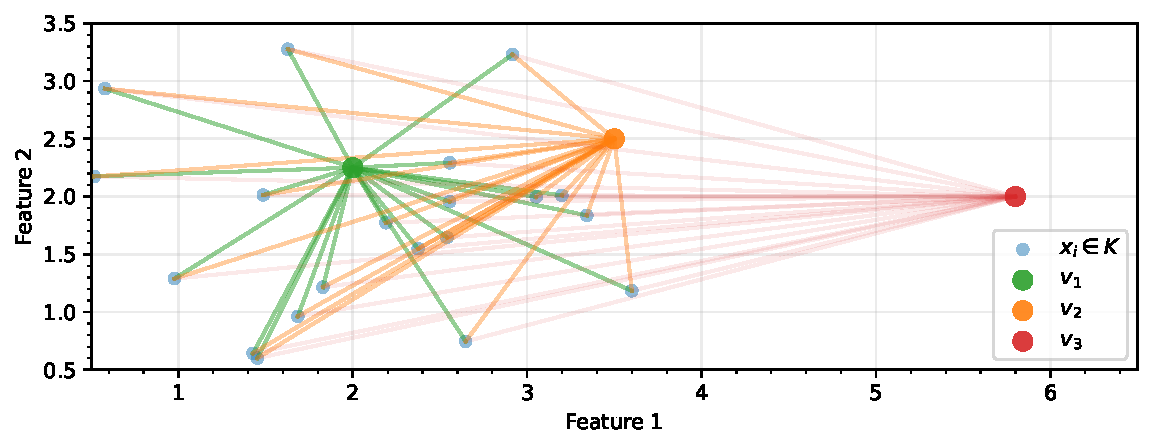
\includegraphics[width=\textwidth]{images/measures/abof-distance.pdf}
    \caption{Idea of the Angle-Based Outlier Factor applied as an outlierness measure.
             Element $v_1$ is located inside the cluster $T$,
             element $v_2$ is on the edge of the cluster $T$
             and element $v_3$ is a distant outlier;
             lines drawn correspond to vectors involved in the outlierness score calculation.}
    \label{fig:abof-idea}
\end{figure}

\begin{figure}[t]
    \centering
    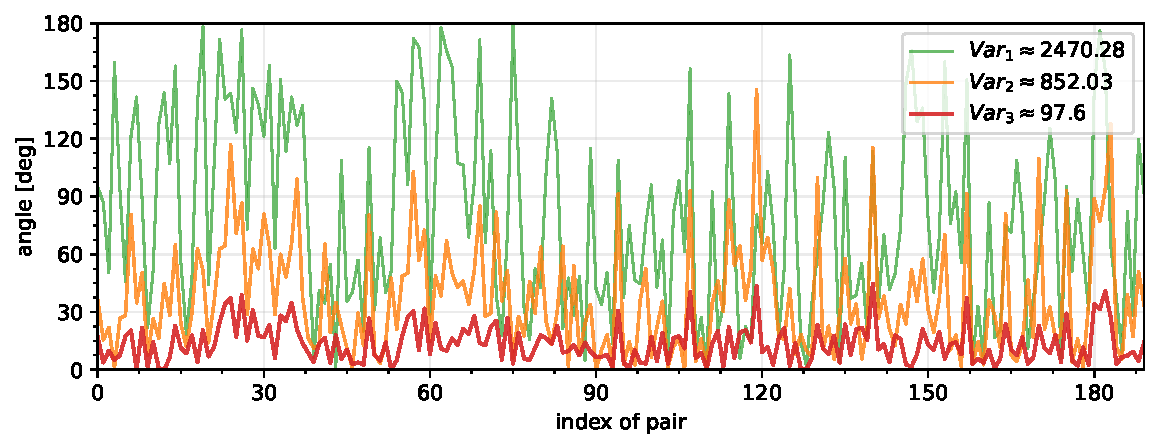
\includegraphics[width=\textwidth]{images/measures/abof-angles.pdf}
    \caption{Ranges of angles between vectors observed for various examined examples
             (typical point – $v_1$, edge point – $v_2$, outlier – $v_3$).
             For $20$ elements in cluster $T$, there are $190$ unique pairs in total,
             so $190$ angles possible for each of points $v_1$, $v_2$ and $v_3$.
             Highest variance is observed for an inlier, lowest variance in case of an outlier.}
    \label{fig:abof-angles}
\end{figure}

The Angle-Based Outlier Factor (ABOF/ABOD), proposed by Kriegel et al. \cite{Kriegel-2008}, is an anomaly detection technique that relies on the analysis of angles between feature vectors to determine whether the data is an outlier or not. Because of relying primarily on angles, instead of e.g., Euclidean distances, it is claimed to be effective even for applications in high-dimensional spaces.

Figure \ref{fig:abof-idea} illustrates the intuitive idea behind the algorithm. For any data point $v$ in the feature space $\mathbb{R}^d$ and a given data cluster $T$, there can be two vectors constructed between the point $v$ and points $x_1$, $x_2$ randomly selected from the cluster $T$. Then, the~angle $\alpha$ (or the value of $\cos(\alpha)$) between the constructed vectors may be calculated.

If the point $v$ is located within the data cluster $T$, then a wide spectrum of angles values may be observed, i.e., both acute and obtuse angles, as presented in figure \ref{fig:abof-angles}. Contrary, when the point $v$ is an outlier, a dominant number of acute angles with small variability of values shall be observed.

Mathematically this can be quantified by calculating the variance of angles values between the given data point $v$ and all possible pairs of points from the target cluster $T$. If the variance is high, i.e., a wide spectrum of angles is observed, the given data point is not an outlier. If the variance is low, the data point is likely to be an outlier.

Let $P$ be the set of all unique pairs $(x_1, x_2)$ – combinations of elements from the target cluster $T$. Then the outlierness score for a given vector $v$ can be calculated as
\begin{equation}
    ABOF(v, T) = \mathrm{Var}\left\{
        ~
        \forall (x_1, x_2) \in P:
        ~
        \frac{
            \vv{x_1 - v} ~\cdot~ \vv{x_2 - v}
        }{
            \norm{\vv{x_1 - v}}^2 \cdot \norm{\vv{x_2 - v}}^2
        }
        ~
    \right\}.
    \label{eq:abof}
\end{equation}

It shall be noticed that because all unique pairs from cluster $T$ are being considered, the computational complexity of the original algorithm is like $\mathcal{O}(n^3)$, hence for large datasets it rapidly becomes time ineffective. Therefore, even the original paper \cite{Kriegel-2008} additionally proposes variants of ABOF: approxABOF and LB-ABOF, that are faster to compute, based on various approximations, e.g., by subsampling the cluster $T$ to consider only $T$ nearest neighbors of point $v$, at the risk of lower accuracy.

In addition it can be observed that in equation \ref{eq:abof} the function formula is not based solely on the angular measure, because considering the scalar/dot product definition,
\begin{equation}
    \vv{v_1} \cdot \vv{v_2}
    =
    \norm{\vv{v_1}} \cdot \norm{\vv{v_2}} \cdot \cos(\alpha),
    \label{eq:dotproduct}
\end{equation}
the original formula \ref{eq:abof} may be therefore presented in a following alternative form,
\begin{equation}
    ABOF(v, T) = \mathrm{Var}\left\{
        ~
        \forall (x_1, x_2) \in P:
        ~
        \frac{
            \cos( \angle (\vv{x_1 - v}, \vv{x_2 - v}) )
        }{
            \norm{\vv{x_1 - v}} \cdot \norm{\vv{x_2 - v}}
        }
        ~
    \right\},
    \label{eq:abof-alt}
\end{equation}
where $\angle (\vv{x_1 - v}, \vv{x_2 - v})$ denotes the angle between vectors $\vv{x_1 - v}$ and $\vv{x_2 - v}$. This makes it visible that the original algorithm actually takes into account the angles that are normalized by the product of the length of the difference vectors \cite{Kriegel-2008}. When the analyzed point $v$ is far from the cluster $T$, the calculated angles are therefore contributing less to the outcome score value. Hence, literature \cite{Walkowiak-2018-asmbi} also discusses the purely angle-based variants without such additional scaling, that turns more accurate in some cases,
\begin{equation}
    ABOF2(v, T) = \mathrm{Var}\left\{
        ~
        \forall (x_1, x_2) \in P:
        ~
        \cos( \angle (\vv{x_1 - v}, \vv{x_2 - v}) )
        ~
    \right\}.
    \label{eq:abof2}
\end{equation}

During the research the own implementation (Section \ref{section:pyopenset}) was used, based on the description from the original article \cite{Kriegel-2008}. For convenience, the returned values were inverted, so the greater values indicate that data more likely to be outliers.

\subsection{Euclidean distance}
\label{section:Euclidean}

\begin{figure}[t]
    \centering
    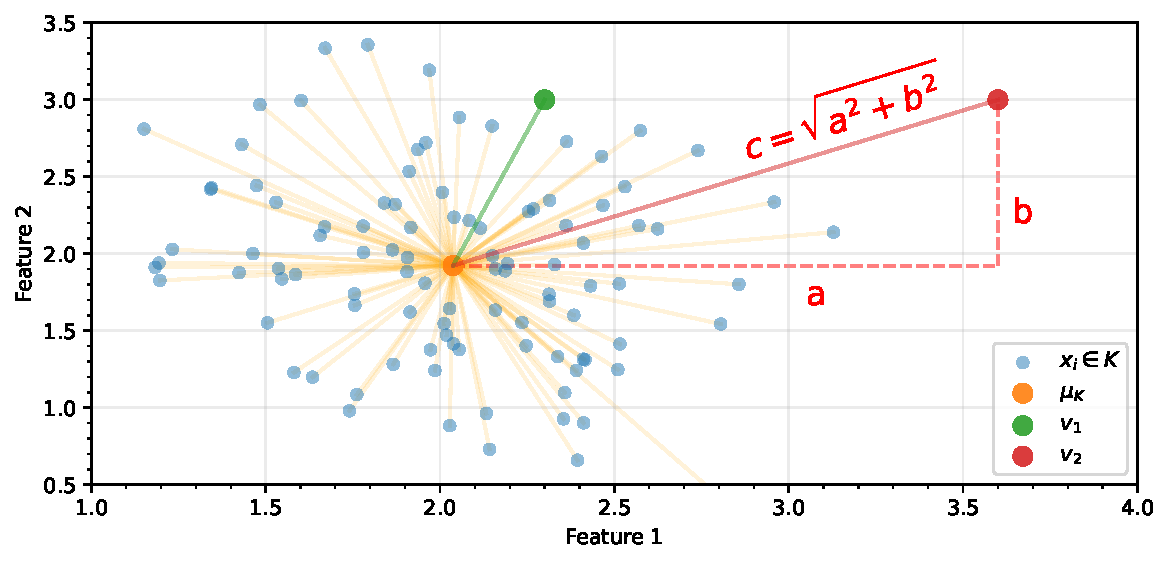
\includegraphics[width=\textwidth]{images/measures/euclidean-distance.pdf}
    \caption{Idea of the Euclidean distance applied as an outlierness measure. \\
             The location $\mu_T$ of the cluster $T$ center is identified and then involved
             in calculation of~the~outlierness scores (Minkowski metric of order $2$) for elements $v_1$ and $v_2$.}
    \label{fig:ed-idea}
\end{figure}

The Euclidean distance is an intuitive baseline method for quantifying the similarity based on the distance. In this approach, the data cluster $T$ is represented by a middle point $\mu_{T}$, calculated as an average of all ($n_{T} = \abs{T}$) feature vectors $x_i$, $x_i \in T$,
\begin{equation}
    \mu_{T} = \frac{1}{n_{T}} \cdot \sum_{i=1}^{n_{T}} x_i
    ~.
    \label{eq:mu_T}
\end{equation}

The outlierness score for a given vector $v$ against the data cluster $T$ is then calculated as the Minkowski distance of order $2$ in $\mathbb{R}^d$ space between the $v$ and point $\mu_{T}$ location,
\begin{equation}
    ED(v, T) = \norm{\vv{v - \mu_{T}}}
    .
    \label{eq:ed}
\end{equation}

Figure \ref{fig:ed-idea} presents the idea of leveraging such simple method for outlier detection. Any element $v$ that is further than acceptable threshold can be marked as outlier ($v_2$), wheres object at typical distance is considered as in-distribution ($v_1$). This approach is suitable as long as the data are evenly distributed on all axes in $\mathbb{R}^d$ space and also not affected by any correlation. Otherwise the risk of spurious ID/OOD label assignment increases, especially in high-dimensional feature spaces.

During the research the implementation from the SciPy library \cite{SciPy-NMeth} was utilized.

\subsection{Integrated Rank Weighted Depth}
\label{section:IRWD}

\begin{figure}[t]
    \centering
    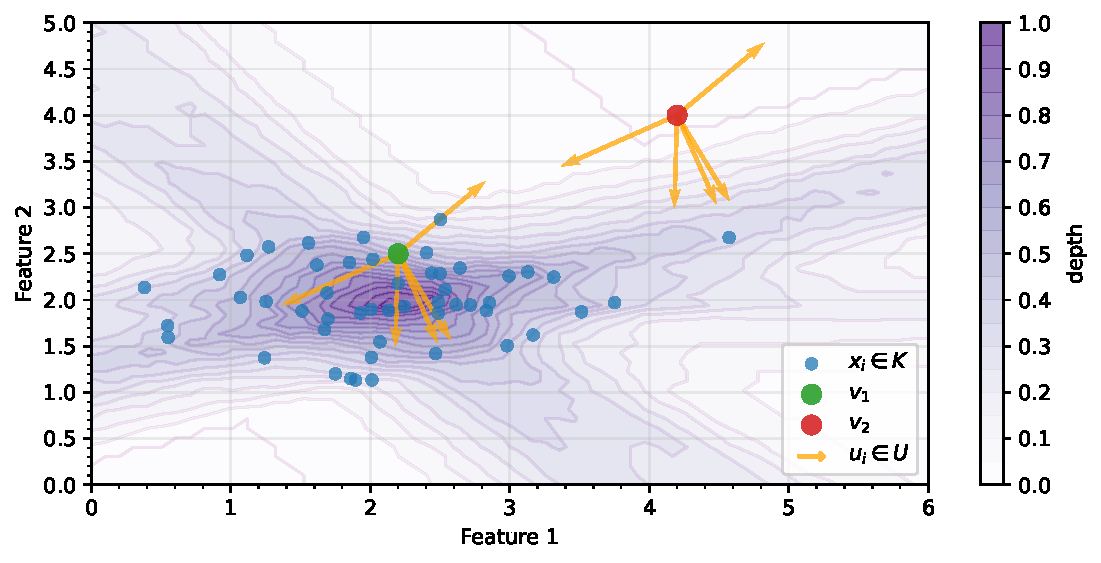
\includegraphics[width=\textwidth]{images/measures/irwd-distance.pdf}
    \caption{Idea of the Integrated Rank Weighted Depth applied as an outlierness measure.
             The contour plot is used to visualize the depths calculated for cluster $T$.
             Point $v_1$ is located in the region surrounded by cluster $T$ points (high depth),
             while point $v_2$ is an outlier (low depth value). The projection vectors $u_i$ involved in depth calculation are drawn for reference. The depth values are normalized for convenience.}
    \label{fig:irwd-idea}
\end{figure}

\begin{figure}[t]
    \centering
    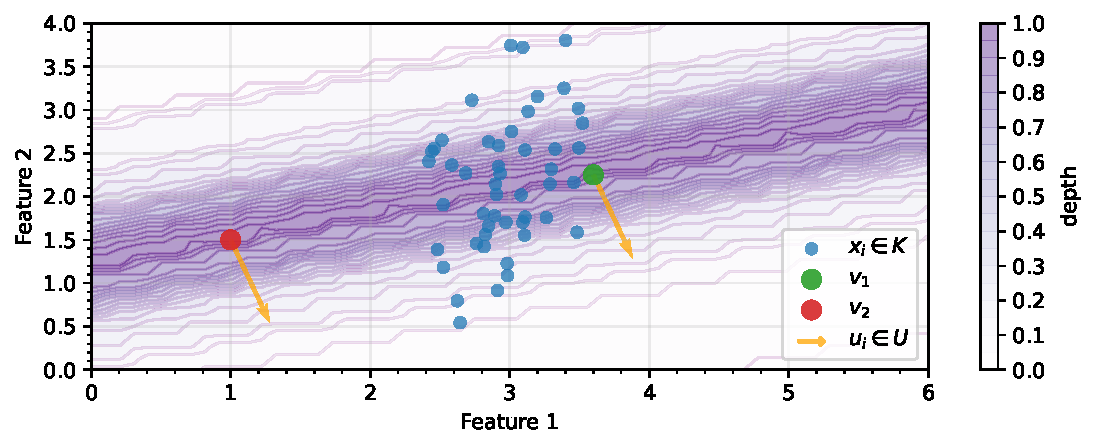
\includegraphics[width=\textwidth]{images/measures/irwd-issue.pdf}
    \caption{The IRWD algorithm identifying spurious correlation due to $n_{proj} < d$.\\
             In this case, element $v_2$ is considered as close to the cluster $T$ as the element $v_1$.
             Utilizing more projection vectors $u_i$ would help mitigating the problem.}
    \label{fig:irwd-issue}
\end{figure}

The Integrated Rank Weighted Depth, published by Ramsay et al. \cite{Ramsay-2019}, is another method of quantifying the outlierness score. It utilizes the Monte Carlo-like approach and considers angles between feature vectors for producing a representation of the known/training set, with the similarity then determined using so called depth of data.

First, a collection $U$ of $n_{proj}$ number of projection vectors $u_j$ is created by randomly selecting directions from a unit hyper-sphere in $\mathbb{R}^d$ space. Then, a representation of known data cluster $T$ is prepared by computing matrix $M$ of size $n_{T} \times n_{proj}$, containing the scalar products between each feature vector $x_i \in T$ and projection vector $\vv{u_j} \in U$,
\begin{equation}
    M[i, j] = x_i \cdot u_j
    ~.
    \label{eq:irwd-M}
\end{equation}

Each $i$-th row in matrix $M$ corresponds to the feature vector $x_i$ of cluster $T$, while each $j$-th column corresponds to the scalar products values obtained for the projection vector $u_j$. Hence, there are $n_{T}$ rows and $n_{proj}$ columns; the $M[i, j]$ component is a~value of the scalar product between vectors $x_i$ and $u_j$.

To calculate the outlierness score for a given vector $v$ against the data cluster $T$, the next step to compute the values of scalar products between $v$ and the projection vectors $u_j \in U$, then subtracting the resulting values from the representation matrix $M$,
\begin{equation}
    M_v[i, j] = M[i, j] - v \cdot u_j
    ~.
    \label{eq:irwd-M_v}
\end{equation}

The resulting matrix $M_v$ is processed column-wise, which corresponds to analyzing results obtained for each projection vector $u_j$. For each column, the number of positive and negative values is counted and the lower number is selected. Finally, the outlierness score is calculated as a sum of selected numbers, divided by the number of $M_v$ elements,
\begin{equation}
    IRWD(v, T)
    =
    \frac{1}{n_{T}}
    \cdot
    \frac{1}{n_{proj}}
    \cdot
    \sum_{j=1}^{n_{proj}}
    \min\big\{
        ~
        \mathrm{count}\{M[*,j] \le 0\}
        ~,~
        \mathrm{count}\{M[*,j] > 0\}
        ~
    \big\}
    ~.
    \label{eq:irwd}
\end{equation}

Intuitively, the values of $M_v$ matrix correspond to the distances and locations of each feature vector $x_i$ in relation to the given $v$ while looking along the direction $u_j$. In~other words, when considering a plane defined by a point $v$ and a vector $u_j$, the positive value of $M_v[i,j]$ means that given $x_i$ is in front/above that plane, while the negative value means the $x_i$ is behind such plane. Note that the actual individual distance itself is not relevant, there matters only the location that is linked to the sign (positive/negative) of the distance value. The score gets maximized, if there is an equal number of elements $x_i$ on both sides of the plane. Hence, the idea of the data depth emerges as a way of characterizing and localizing the center of a~distribution, which is promised to be suitable especially for non-Gaussian distributions, where only the traditional mean and median may not provide reliable understanding of data spread.

The high depth value indicates that a data point $v$ lies within the central region of the data cluster $T$, surrounded by neighbors. Contrary, low depth value suggests that a~point is located on the outskirts of the data distribution, potentially indicating that the $v$ may by an outlier. Figure \ref{fig:irwd-idea} illustrates both such cases with the random projection vectors $u_i$ drawn for the reference as well.

It is worth to notice that the chosen number of random projection vectors, $n_{proj}$, impacts the outcome of IRWD significantly. Especially, with $n_{proj}$ lower than the dimension of $\mathbb{R}^d$ space, i.e., $n_{proj} < d$, there is a risk of identifying spurious correlations in data. Example of the such case was presented in the figure \ref{fig:irwd-issue}, where both in-distribution data ($v_1$) and the out-of-distribution sample ($v_2$) are ranked with the same depth score.

During the research the own implementation (Section \ref{section:pyopenset}) was used, based on the description from the the NeurIPS publication \cite{Colombo-2022}. For convenience, the returned values were inverted, so the greater values indicate that data more likely to be outliers.

\subsection{k-Nearest Neighbors}
\label{section:kNN}

\begin{figure}[t]
    \centering
    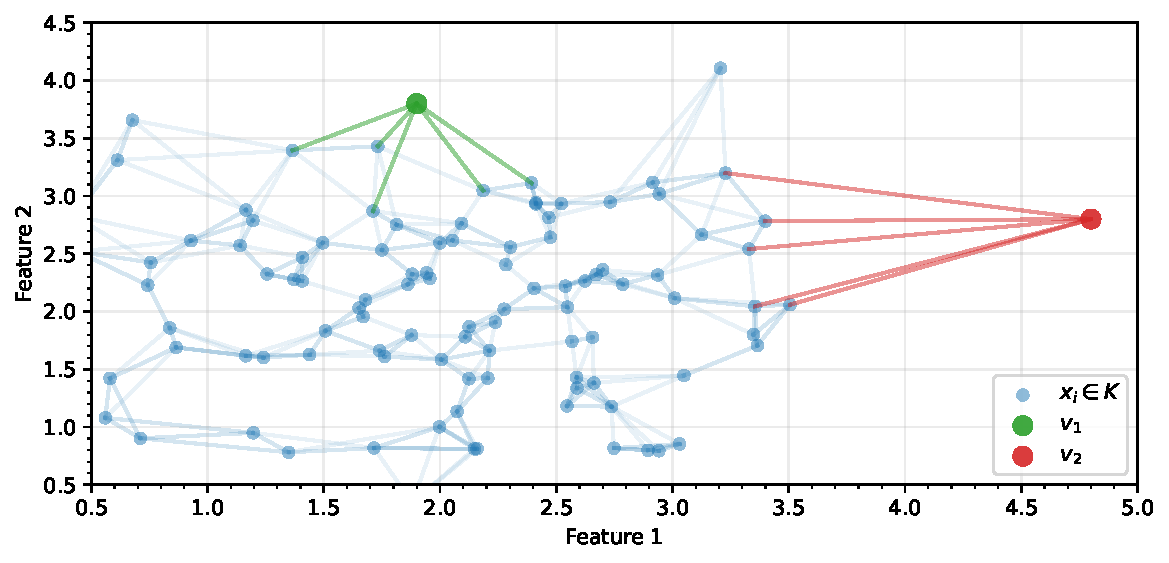
\includegraphics[width=\textwidth]{images/measures/knn-distance.pdf}
    \caption{Idea of the k-Nearest Neighbors applied as an outlierness measure. \\
             The lines drawn connects elements to their $k=5$ closest neighbors.
             Element $v_1$ is~located close to the cluster $T$, so average distance
             to it's closest neighbors is~lower~than for element $v_2$ that is located farther.}
    \label{fig:knn-idea}
\end{figure}

The k-Nearest Neighbors is a well defined, fundamental algorithm of the machine learning~\cite{Hastie-2009}, that is useful in variety of tasks, such as in clusterization and classification. It was recently proposed as a state-of-the-art out-of-distribution detector \cite{Sun-2022}.

The core concept assumes the identification of given $k$ number of elements from a~known set $T$ that are closest neighbors of a given element $v$. Such identification can be performed by using one from a number of possible underlying algorithms, for~example a~naive brute-force search or by utilizing sophisticated data structures, like with k-dimensional tree \cite{Bentley-1975}\cite{Brown-2015} or ball tree algorithm \cite{Omohundro-1989}\cite{Liu-2006}. Also, for distance calculation, there may be any of the known metrics involved, such as the Manhattan/L1 distance or the general Minkowski metric; commonly the standard Euclidean distance is used \cite{Singh-2013}.

In applications for outlier detection, there are two main approaches proposed in the literature. First solution relies on selecting the distance to the $k$-th neighbor as the outlierness score, i.e., the highest distance among all $k$ neighbors around given $v$,
\begin{equation}
    {kNN}_{I}(v, T)
    =
    \max\big\{
        ~
        \forall x_i \in N_k(v, T): ~ \norm{\vv{v - x_i}}
        ~
    \big\}
    ,
    \label{eq:kNN-max}
\end{equation}
where $N_k(v, T)$ is a function that returns the set containing $k$ number of elements $x_i$ from cluster $T$ that are closest to $v$. The second approach relies on calculating the average distance to all of $k$ considered neighbors,
\begin{equation}
    {kNN}_{II}(v, T)
    =
    \frac{1}{k}
    \cdot
    \left(
        ~
        \sum_{x_i \in N_k(v, T)} \norm{\vv{v - x_i}}
        ~
    \right)
    .
    \label{eq:kNN-avg}
\end{equation}

Typically, the high values of the calculated outlierness score, above certain threshold, indicate that given feature vector $v$ is far from all samples present in training cluster $T$, i.e., it is an outlier. Respectively, low values of the score indicate that the $v$ is not distant from known examples, hence it is an inlier.

Figure \ref{fig:knn-idea} illustrates the representation of example cluster $T$ from the kNN algorithm's perspective, along with in-distribution sample ($v_1$) and outlier ($v_2$). The key advantage of the algorithm is that no arbitrary assumption on the data distribution is required, as it relies purely on the proximity of the neighbor points. On the other hand, the algorithm is therefore sensitive to any incorrectly labeled entries in the training dataset that may lead to further spurious assignments.

It shall be noticed that for the very, very large datasets, containing huge number of high-dimensional feature vectors ($n \sim 1\,000\,000\,000$), the process of identifying the nearest neighbors can become slow and the model may be difficult to fit into RAM (Random Access Memory). To~overcome this, companies that deal with searching through such enormous amounts of data on daily basis presented recently their dedicated solutions for this problem. The Faiss library\footnote{\url{https://github.com/facebookresearch/faiss}} \cite{Douze-2024}, developed mainly by Fundamental AI Research group at Meta (formerly Facebook), is an example solution that utilizes the product quantization based approach for approximate nearest neighbor search \cite{Jegou-2011}. Another example is Annoy library\footnote{\url{https://github.com/spotify/annoy}} (Approximate Nearest Neighbors Oh Yeah), developed by Erik Bernhardsson and used at Spotify for music recommendations, that supports file-based indexes mapped into RAM that can be effectively shared between multiple system processes.

During the research the implementation from the scikit-learn library \cite{scikit-learn} was used.

\subsection{Local Outlier Factor}
\label{section:LOF}

\begin{figure}[t]
    \centering
    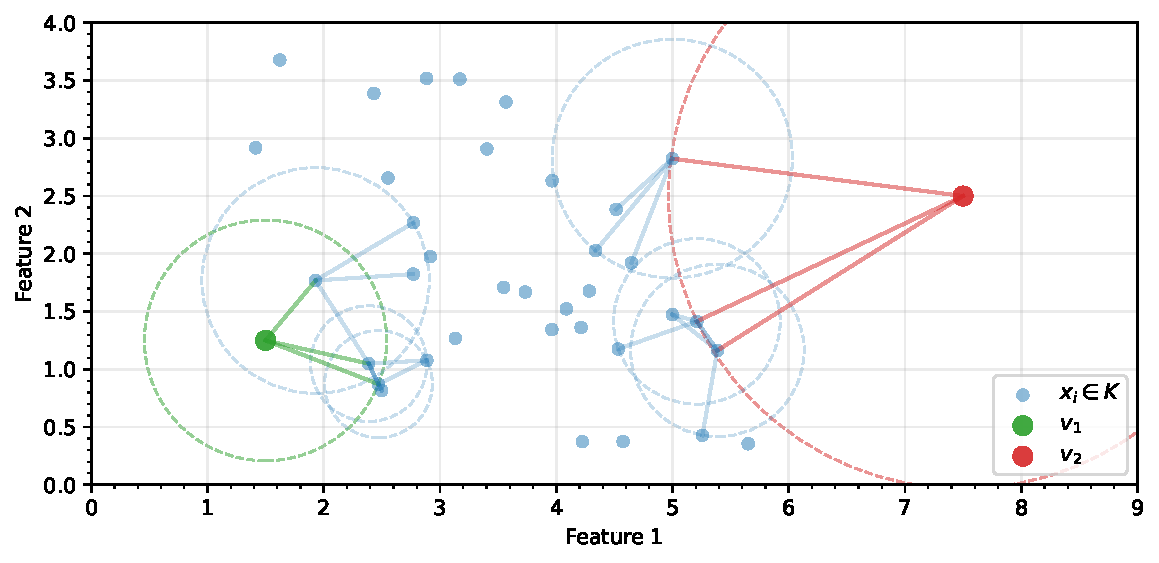
\includegraphics[width=\textwidth]{images/measures/lof-distance.pdf}
    \caption{Idea of the Local Outlier Factor applied as an outlierness measure. \\
             The $k=3$ closest neighbors are considered when identifying the reachability distances (represented as the radiuses of circles).
             For element $v_1$ the reachability distance is~similar as for it's neighbors,
             whereas for element $v_2$ it is significantly greater.}
    \label{fig:lof-idea}
\end{figure}

The Local Outlier Factor (LOF), originally described by Breunig et al. \cite{Breunig-2000}, is a well-established algorithm widely used to detect abnormal data in high-dimensional spaces. It is based on the concepts of so called reachability distance and local reachability density. Instead of considering the global data distribution, it aims to identify outliers by analyzing only the local neighborhood. Hence, it can be considered as an extension of the k-Nearest Neighbors algorithm.

Let $N_k(v, T)$ be a function that returns the set containing $k$ number of elements $x_i$ from cluster $T$ that are closest to $v$. The base concepts utilized by LOF are therefore defined as follows. First, the $kdist(v, T)$ is defined as the distance from given $v$ to its $k$-th neighbor from the cluster $T$,
\begin{equation}
    kdist(v, T)
    =
    \max\big\{
        ~
        \forall x_i \in N_k(v, T): ~ \norm{\vv{v - x_i}}
        ~
    \big\}
    .
    \label{eq:kdist}
\end{equation}

Then, the reachability distance of element $v$ with respect to the element $x$ and cluster $T$ is defined as either the true distance between $v$ and $x$, or as the $kdist(x, T)$ distance of element $x$, whichever turns greater,
\begin{equation}
    rd_k(v, x, T)
    =
    \max\big\{
        ~
        kdist(x, T),
        ~
        \norm{\vv{v - x}}
        ~
    \big\}
    .
\end{equation}

Successively, the local reachability density for an element $v$ with respect to the given cluster $T$ is defined as the inverse of the average reachability distance of element $v$ and its $k$ neighbors from set $T$,
\begin{equation}
    lrd_k(v, T)
    =
    \frac{
        k
    }{
        \sum_{x_i \in N_k(v, T)} rd_k(v, x_i, T)
    }
    ~.
\end{equation}

Finally, the outlierness score for a given vector $v$ against the target data cluster $T$ is calculated as an average local reachability density of $k$ neighbors of $v$, divided by the local reachability density of the $v$ element,
\begin{equation}
    LOF(v, T)
    =
    \frac{
        \sum_{x_i \in N_k(v, T)} lrd_k(x_i, T)
    }{
        k \cdot lrd_k(v, T)
    }
    ~.
\end{equation}

Figure \ref{fig:lof-idea} illustrates the idea of Local Outlier Factor algorithm. Intuitively, the algorithm compares the radiuses of circles corresponding to the reachability distances of the analyzed points and their $k$ closest neighbors. Shall these radiuses be similar to their neighbors ones ($v_1$, score $LOF \approx 1$), the point can be considered an inlier. On~the~other hand, when the radius at analyzed point is much greater ($v_2$, $LOF \gg 1$), then such point is likely an outlier. High score value means a given point $v$ is relatively far from the cluster, as there is low density of points in the surrounding area (inverse of reachability distance).

It is worth to mention that, similarly to k-Nearest Neighbors algorithm, the Local Outlier Factor does not require any \textit{a priori} assumption on the data distribution, since it identifies the outliers only by analyzing the local surroundings of data. Hence LOF algorithm represents so called non-parametric approach to anomaly detection.

The LOF algorithm captures the intuition that outliers are isolated points, while denser regions of data are related with areas typical for a given distribution. It can be adapted to handle different distance metrics as well. Nevertheless, the value of $k$ affects the sensitivity of the algorithm to any local variations in density. However, the algorithm can be computationally expensive for large datasets due to the complexity of finding neighbors in data.

During the research the implementation from the scikit-learn library \cite{scikit-learn} was utilized.

\subsection{Mahalanobis distance}
\label{section:Mahalanobis}

\begin{figure}[t]
    \centering
    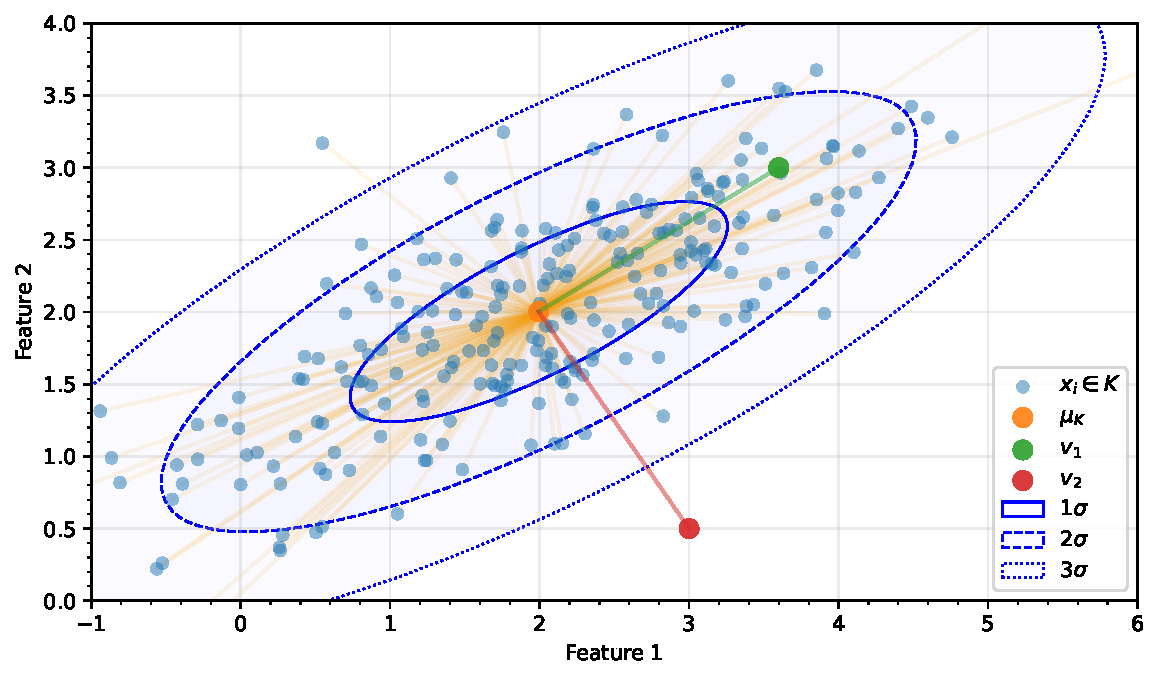
\includegraphics[width=\textwidth]{images/measures/mahalanobis-distance.pdf}
    \caption{Idea of the Mahalanobis distance applied as an outlierness measure.
             The~confidence ellipses indicate the distribution properties of cluster $T$;
             the marked areas correspond to regions in which about 68.2\%, 95.4\% and 99.7\%
             data are located. Despite that elements $v_1$ and $v_2$ have similar
             Euclidean distances from the cluster center $\mu_K$, only the element $v_1$
             is located in the more typical region, still surrounded by~elements $x_i \in T$,
             while $v_2$ shall be considered an outlier in this case.}
    \label{fig:md-idea}
\end{figure}

The Mahalanobis distance is one of the state-of-the-art solutions for performing out-of-distribution detection nowadays – often proposed directly as a method \cite{Lee-2018}\cite{Fort-2021}\cite{Du-2022}, mentioned in benchmarks \cite{Tajwar-2021}\cite{Zhou-2021}\cite{Podolskiy-2022}\cite{Yang-2022} or used as a baseline when compared with new techniques \cite{Liu-2020}\cite{Colombo-2022}\cite{Sun-2022}. It was originally described in 1936 by an Indian statistician P. C. Mahalanobis in \cite{Mahalanobis-1936} as a generalized distance metric for a~normally distributed multidimensional data, i.e., multivariate Gaussian distribution. It is claimed to be effectively applicable to high-dimensional data and promised to be more accurate than other measures, especially if there are correlated features in data.

It is an example of parametric method for outlier detection, that assumes in advance a specific characteristic of the data distribution, here: MVN (Multivariate Normal distribution); and the parameters of such a distribution, such as vector of means ($\mu$) and the covariance matrix ($\Sigma$), are estimated based on a provided training dataset.

The outlierness score for a given vector $v$ against the data cluster $T$ is calculated as
\begin{equation}
    MD(v, T) = \sqrt{
        (\vv{v - \mu_{T}})^{\top}
        \cdot
        \Sigma_{T}^{-1}
        \cdot
        (\vv{v - \mu_{T}})
    }.
    \label{eq:md}
\end{equation}

The $\mu_{T}$ represents the center of cluster $T$ – it is a vector of means of each variable ($\mu_{T} \in \mathbb{R}^d$). The $\Sigma_{T}^{-1}$ corresponds to the inverse of the covariance matrix $\Sigma_{T}$ calculated for the cluster $T$. In statistics the $\Sigma_{T}^{-1}$ element is also known as the precision matrix \cite{Wasserman-2010} (or concentration matrix).

High output values indicate the larger distance from the distribution center, suggesting that $v$ is potential outlier. Contrary, low values imply that $v$ resides close to the center of cluster $T$, conforming more to the data distribution and not being an outlier.

It shall be noticed that without the additional factor $\Sigma_{T}^{-1}$ the formula \ref{eq:md} would be an equivalent to the classical Euclidean distance in $\mathbb{R}^d$ space. Hence, the  $\Sigma_{T}^{-1}$ element can be interpreted as a scaling factor of the space where the distance is measured. In other words, the distance between analyzed point $v$ and the cluster center $\mu_{T}$ is adjusted to account the distribution shape, as the straight Euclidean distance along one axis can be more typical than the same straight distance along the axis where the data are more concentrated.

Figure \ref{fig:md-idea} illustrates such example, where the element $v_1$ can be considered as belonging to the data distribution, while the element $v_2$ is an outlier, despite the fact that both elements have similar Euclidean distance from the distribution center $\mu_{T}$.

It must be taken into account that as the estimation of the covariance matrix is required, fitting the algorithm to the training data can be computationally expensive if the datasets is large (i.e., big number of samples, high dimension of feature vectors). It is worth to notice that the typically used algorithms, like Maximum-Likelihood Estimation (MLE), are sensitive to the presence of any outliers in the dataset, so in cases where any contamination in the dataset may be present the literature suggests utilizing other techniques, such as the Minimum Covariance Determinant estimator \cite{Rousseeuw-1984}\cite{scikit-learn}\footnote{\scriptsize\url{https://scikit-learn.org/stable/auto_examples/covariance/plot_mahalanobis_distances.html}}.

Additional requirement for the inverse of covariance matrix $\Sigma^{-1}$ is that it must be positive-semidefinite and symmetric. The condition is that for a symmetric real matrix $M$ of dimension $d \times d$ there exist no such vector $v \in \mathbb{R}^d$ that would produce a negative result of a product $v^\top \cdot M \cdot v$; formally
\begin{equation}
    M = M^\top
    ~
    \land
    ~
    \forall v \in \mathbb{R}^d: v^\top \cdot M \cdot v \geq 0
    ~
    \Longleftrightarrow
    ~
    M ~ \text{is positive-semidefinite}.
    \label{eq:M-positive-semidefinite}
\end{equation}
When that condition is met, the $M$ can be expressed as a product of a lower triangular matrix $A$ and its transpose $A^\top$, i.e., $M = A^\top \cdot A$, known as the Cholesky decomposition \cite{Higham-1990}. Then, the product $v^\top \cdot M \cdot v$ is equal to the length of the vector $v$ transformed by the matrix $A$,
\begin{equation}
    v^\top \cdot M \cdot v
    =
    v^\top \cdot A^\top \cdot A \cdot v
    =
    (A \cdot v)^\top \cdot (A \cdot v)
    =
    \norm{A v}
    .
    \label{eq:M-length}
\end{equation}
Intuitively, this condition ensures that the output of formula \ref{eq:md} is not negative and can be interpreted as a distance metric. However, this condition cannot be satisfied when the number of samples $n$ is lower than features space dimension $d$ or the rank of the matrix $\Sigma^{-1}$ is lower than $d$ (as a result of highly correlated features or linearly dependent columns in the data – observed during research for ViT representation [section \ref{section:ViT}], further detailed study is needed).

Difficulties in practical applications for high-dimensional data involve the requirement of providing the sufficient number of training samples to fit the distribution model, i.e.~at~least $n_{T} \geq d$ and ideally $n_{T} \gg d$, for stable estimation of the covariance matrix $\Sigma_{T}$. However, for common datasets, such as \textit{ImageNet-1k} \cite{Russakovsky-2015}, there are underrepresented categories present that not satisfy this requirement, especially for large models with $d > 1000$ number of features, e.g., ResNet ($d = 2048$ features), ConvNeXT ($d = 1536$ features), EfficientNet ($d = 1280$ features). Hence, the approaches emerged, such as proposed in literature \cite{Lee-2018}\cite{Tajwar-2021}, to calculate the single covariance matrix $\Sigma$ using the whole training dataset for all classes as input, while still distinguishing means $\mu_{T}$ per data cluster during the distance calculation. This approach is sometimes called as utilizing the pooled covariance matrix \cite{Johnson-2007}\cite{Raninen-2022} and so the outlierness score can be calculated here for $m$ classes and vector of labels $y$ as follows:
\begin{equation}
    \Sigma
    =
    \frac{1}{n}
    \sum_{c=1}^{m}
    \sum_{i: y_i = c}^{n_c}
    (\vv{x_i - \mu_{c}})
    \cdot
    (\vv{x_i - \mu_{c}})^{\top}
    ,
    \label{eq:mdp-sigma}
\end{equation}
\begin{equation}
    MDP(v, T) = \sqrt{
        (\vv{v - \mu_{T}})^{\top}
        \cdot
        \Sigma^{-1}
        \cdot
        (\vv{v - \mu_{T}})
    }.
    \label{eq:mdp}
\end{equation}

During the research the implementation from the SciPy library \cite{SciPy-NMeth} was utilized.

\subsection{Standardized Euclidean distance}
\label{section:SEuclidean}

\begin{figure}[t]
    \centering
    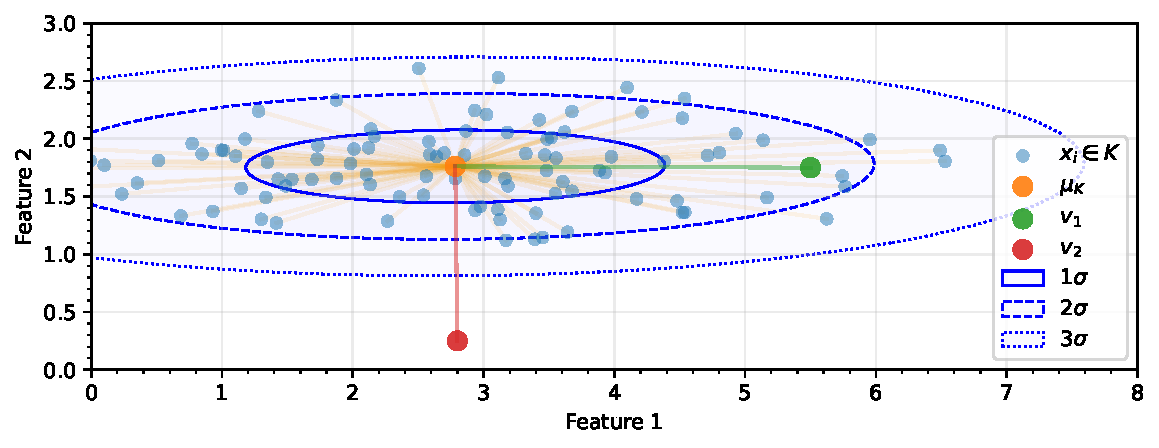
\includegraphics[width=\textwidth]{images/measures/seuclidean-distance.pdf}
    \caption{Idea of the Standardized Euclidean distance applied as an outlierness measure.
             Cluster $T$ displays the heterogeneous spread along the axes – higher variance
             on feature 1 and lower variance on feature 2. Considering the different variances,
             after scaling the axes ($\sigma_1 \approx 1.5$, $\sigma_2 \approx 0.3$),
             the element $v_1$ is located closer to center $\mu_K$ than the element $v_2$
             that is outlier (distance $d_1 \approx \frac{2.7}{1.5} \approx 1.8$,
             distance $d_2 \approx \frac{1.5}{0.3} \approx 5.0$).}
    \label{fig:sed-idea}
\end{figure}

The Standardized Euclidean distance is another measure based on Minkowski metric of order $2$ in $\mathbb{R}^d$ space – a square root of the sum of vector elements to the power of $2$. It considers axes-wise variances to normalize the contributions of each vectors elements when calculating the distance. It can be considered as a compromise between the traditional Euclidean distance, that assumes uniform relevance of all axes, and more general Mahalanobis distance, that estimates the distribution shape using the covariance matrix.

The outlierness score for a given vector $v$ against the data cluster $T$ is calculated as
\begin{equation}
    SED(v, T) = \sqrt{
        \sum_{j=1}^{d}
        \frac{1}{V_{T,j}}
        \cdot
        \left(
            v_{j} - \mu_{T,j}
        \right)^2
    }.
    \label{eq:sed}
\end{equation}

The $V_K$ represents a vector of variances; the $V_{T,j}$ is a variance along $j$-th axis in cluster $T$ and $v_j$ is the $j$-th components of the vector $v$. The $\mu_{T}$ corresponds to the center of the cluster $T$. When the calculated value is high, the given data point is distant from the cluster center and is likely an outlier, while lower values indicate data close to the given cluster.

Similarly to the Mahalanobis distance, it scales the axes to have a uniform, unitary variance. However, contrary to the Mahalanobis distance, the Standardized Euclidean distance does not take into account the correlations between features in the data, assuming those are independent. Because of this, it is much more efficient when utilized in high-dimensional spaces, because no computationally expensive inversion of covariance matrix is necessary to fit the algorithm to the training data, while it still considers the orientation and shape of data distribution.

Furthermore, as discussed in the chapter \ref{chapter:simulations} (section \ref{section:estimation-experiment}), the estimation of variances is much more stable than the estimation of covariances, so a lower method error would be made when the analyzed data are uncorrelated or the correlation of features is negligibly small.

During the research the implementation from the SciPy library \cite{SciPy-NMeth} was utilized.

